% !TEX jobname = thesis
% !TEX output_directory = output

\documentclass[
    accentcolor=tud9c,
    %colorbacktitle,
    ruledheaders=chapter,
    class=book,
    11pt,
    paper=a4,
    bigchapter,
    twoside
]{tudreport}

\usepackage[utf8]{inputenc}
\usepackage[ngerman, english]{babel}
\usepackage{hyperref}
\usepackage{titlesec}

\usepackage{enumitem}
\usepackage{setspace}
\setstretch{1.1}

\usepackage[none]{tocbibind}

% Two commands which could be helpful for you ...
% ... First, a command to handle todos in a simple way
\newcommand{\todo}[1]{{\color{red}{\textbf{TODO: }#1}}}
% ... Second, a command which highlights numbers you need to check.
\newcommand{\checkNum}[1]{{\textcolor{orange}{\textit{#1}}}}
% If you have checked all information in red, change the color to black.
%\newcommand{\checkTitle}[1]{{\textcolor{red}{\textit{#1}}}}
\newcommand{\checkTitle}[1]{{\textcolor{black}{\textit{#1}}}}
\title{Identification and Analysis of unsafe.Pointer Usage Patterns in Open-Source Go Code}
\subtitle{It's dangerous to Go alone. Take *this!\\~}
\author{Johannes Tobias Lauinger}
\reviewer{Prof. Dr.-Ing. Mira Mezini \and Anna-Katharina Wickert, M.Sc. \and Dr. rer. nat. Lars Baumgärtner}
\department{inf}
\institute{Software Technology Group}
\submissiondate{\today}
\examdate{\today}
%\tuprints{urn=1234,printid=12345}
\dedication{To fritz, without which none of this\\would have happened.}

\Metadata{
    title={Identification and Analysis of unsafe.Pointer Usage Patterns in Open-Source Go Code},
    author={Johannes Tobias Lauinger}
}

\maketitle

\setlength{\parindent}{0em}
\setlength{\parskip}{1em}

\titlespacing\section{0pt}{12pt plus 4pt minus 2pt}{0pt plus 2pt minus 2pt}
\titlespacing\subsection{0pt}{12pt plus 4pt minus 2pt}{0pt plus 2pt minus 2pt}
\titlespacing\subsubsection{0pt}{12pt plus 4pt minus 2pt}{0pt plus 2pt minus 2pt}


\begin{document}

%% front page
\pagenumbering{roman}%
\maketitle%
%% declaration
\chapter*{Erklärung zur Abschlussarbeit gemäß § 22 Abs. 7 und § 23 Abs. 7 APB TU Darmstadt }

Hiermit versichere ich, \yourName{}, die vorliegende \yourCourseOfStudies{} gemäß § 22 Abs. 7 APB der TU Darmstadt ohne Hilfe Dritter und nur mit den angegebenen Quellen und Hilfsmitteln angefertigt zu haben. Alle Stellen, die Quellen entnommen wurden, sind als solche kenntlich gemacht worden. Diese Arbeit hat in gleicher oder ähnlicher Form noch keiner Prüfungsbehörde vorgelegen.

Mir ist bekannt, dass im Falle eines Plagiats (§38 Abs.2 APB) ein Täuschungsversuch vorliegt, der dazu führt, dass die Arbeit mit 5,0 bewertet und damit ein Prüfungsversuch verbraucht wird. Abschlussarbeiten dürfen nur einmal wiederholt werden.

Bei der abgegebenen Thesis stimmen die schriftliche und die zur Archivierung eingereichte elektronische Fassung gemäß § 23 Abs. 7 APB überein.

\vspace{2cm}
\hfill \parbox{6cm}{Darmstadt, den \yourSubmissionDate{} \\ \\ \phantom{.}}
\parbox{6cm}{\centering\hrule\medskip \yourName{}}
%
\cleardoublepage%
%% abstract
\chapter*{Abstract}

After \checkNum{one decade} since its first published version, the Go programming language has become a popular and
widely used systems programming language.
It aims to achieve thorough memory and thread safety by using compile-time measures such as a strict type system that
prevents invalid memory access.
However, there is also the \unsafe{} package which allows developers to deliberately circumvent this safety net.
There are a number of legitimate use cases for doing this, for example a low-level network protocol implementation that
needs access to the raw byte representation of some data, or an in-place type conversion saving reallocation costs to
improve efficiency.

Misusing the \unsafe{} API can however lead to security vulnerabilities such as buffer overflow and use-after-free bugs.
This work contributes an analysis of \unsafe{} usage patterns with respect to a security context.
It reveals possible code injection and information leak vulnerabilities in proof-of-concept code as well as common code
usages from real-world code.

To assess the risk of \unsafe{} code in their applications, this work presents \toolGeiger{}, a novel tool to help
developers quantify \unsafe{} usages not only in their project itself but including its dependencies.
Using \toolGeiger{}, we conducted a study on \unsafe{} usage in the top \projsTotal{} most popular open-source Go
projects on \github{}, including a manual study of \numberLabeledCodeSnippets{} individual code samples on how \unsafe{}
is used and for what purpose.
The study shows that \percentageUnsafePackages{} of packages imported by the projects using the Go module system use
\unsafe{}.
\percentageUnsafeProjects{} of the projects use \unsafe{} directly, but \percentageUnsafeTransitiveWithDependencies{}
include \unsafe{} usages through any of their dependencies.
A replication and comparison of a concurrent study by Costa et al.~\cite{costa2020} matches these results.

This work further presents \toolSafer{}, a novel static code analysis tool that helps developers to identify
\checkNum{two} dangerous and common misuses of the \unsafe{} API which were previously undetected with existing tools.
Using \toolSafer{}, we identified \numberBugsFixed{} bugs in real-world code and submitted patches to the maintainers.
An evaluation of the tool shows \goSaferEvaluationDatasetGosaferAccuracy{} accuracy on my data set of labeled \unsafe{}
usages, and \goSaferEvaluationPackagesGosaferAccuracy{} accuracy on a set of manually inspected open-source Go packages.


\chapter*{Zusammenfassung}

Nach \checkNum{einem Jahrzehnt} seit der ersten veröffentlichten Version ist die Programmiersprache Go heute eine
beliebte und weit verbreitete Systemprogrammierungssprache.
Sie strebt Speicher- und Threadsicherheit durch Compiler-Maßnahmen wie ein striktes Typsystem, das
ungültige Speicherzugriffe verhindert, an.
Es gibt allerdings ebenfalls das \unsafe{} Package, eine API die es Entwickler*innen erlaubt, diese
Maßnahmen zu umgehen.
In manchen Fällen kann dies gerechtfertigt sein, beispielsweise bei der Implementierung eines
Netzwerkprotokolls, das direkten Zugriff auf die konkreten Daten benötigt, oder zur Konvertierung von Daten in einen
anderen Typ, ohne diese im Speicher zu kopieren, um so die Effizienz des Programms zu steigern.

Eine falsche Benutzung der \unsafe{} API kann jedoch zu Sicherheitsproblemen wie Buffer Overflows und Use-After-Frees
führen.
Diese Arbeit analysiert Verwendungsmuster von \unsafe{} Code im Hinblick auf Sicherheitsrisiken.
Dabei treten mögliche Code Injection und Information Leak Verwundbarkeiten sowohl in Proof-of-Concepts als auch in
realem Anwendungscode zu Tage.

Um die Risiken durch \unsafe{} Code in Anwendungen abzuschätzen, stellt diese Arbeit \toolGeiger{} vor, ein neues
Werkzeug das Entwickler*innen dabei hilft, \unsafe{} Nutzungen nicht nur in ihren Projekten sondern auch in deren
Abhängigkeiten zu finden.
Mit \toolGeiger{} führen wir eine Studie zur Nutzung von \unsafe{} in den Top \projsTotal{} beliebtesten Open-Source Go
Projekten auf \github{}, inklusive einer manuellen Analyse von \numberLabeledCodeSnippets{} individuellen Codestücken
in Bezug darauf wie und zu welchem Zweck \unsafe{} benutzt wird.
Die Studie zeigt, dass \percentageUnsafePackages{} der Packages, die von Projekten die das Go Modules System
unterstützen, importiert werden, \unsafe{} verwenden.
\percentageUnsafeProjects{} der Projekte nutzen \unsafe{} direkt, und \percentageUnsafeTransitiveWithDependencies{}
enthalten \unsafe{} Code durch ihre Abhängigkeiten.
Eine Replikation sowie ein Vergleich mit einer zeitgleichen Studie von Costa et al.~\cite{costa2020} bestätigt diese
Ergebnisse.

Weiterhin präsentiert diese Arbeit \toolSafer{}, ein neues statisches Analysewerkzeug, das Entwickler*innen hilft,
\checkNum{zwei} gefährliche und häufig vorkommende inkorrekte Verwendungen der \unsafe{}, die mit bisher existierenden
Tools nicht gefunden werden, zu identifizieren.
Mittels \toolSafer{} konnten wir \numberBugsFixed{} Fehler in realem Code finden und entsprechende Patches einreichen.
Eine Evaluation des Tool ergibt eine Accuracy von \goSaferEvaluationDatasetGosaferAccuracy{} auf meinem Datensatz von
\unsafe{} Codezeilen, und \goSaferEvaluationPackagesGosaferAccuracy{} Accuracy auf händisch analysierten Open-Source
Go Packages.
%
\cleardoublepage%
%% table of contents
\renewcommand\contentsname{Table of Contents}%
\tableofcontents%
\cleardoublepage%
\pagenumbering{arabic}%

%% content chapters
%% -----------------------------------------------------------------------------

\chapter{Introduction}\label{ch:introduction}


%% -----------------------------------------------------------------------------

\section{Motivation}\label{sec:motivation}

In today's modern society, ...

Modern programming languages like Rust and Go have mechanisms to protect potential
unsafe usages, e.g., dereferences of raw pointers or modifying static variables. Thus, it is
recommended to avoid unsafe usages. However, if a developer wants to avoid unsafe
usages and potential security vulnerabilities caused by these usages, they do not only need
to check their code but also their dependencies.

To provide a developer the power to understand the unsafe usages within their code base,
tools like cargo-geiger~\cite{cargogeiger} exists. Unfortunately, such a tool does not exist by today for Go.
Thus, an in-depth analysis of how many Go projects include direct and indirect unsafe
usages and if these projects are vulnerable does not exist, e.g., to buffer overflows~\cite{larochelle2001, alnaeli2017, wang2020}.
Within this work, the aim is to develop a tool, probably based on go vet~\cite{govet}, that can identify
unsafe usages in Go projects - similar to cargo-geiger. Based on this tool, the thesis should
evaluate how common unsafe usages in Go are and try to analyze if vulnerabilities caused
by unsafe usages exist.

\begin{figure}
    \centering
    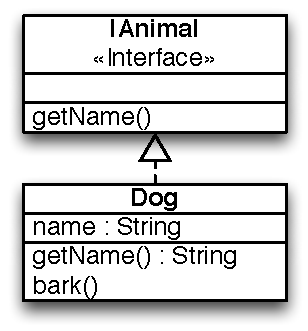
\includegraphics[width=4cm]{assets/images/uml}
    \caption{Sample UML Diagram}
    \label{fig:uml_example}
\end{figure}



%% -----------------------------------------------------------------------------

\section{Contributions}\label{sec:contributions}

The contributions of this thesis are:

\begin{enumerate}
    \item A large-scale study of unsafe code usage in the 500 most popular open-source Go projects,
    including the identification of (three) main areas of danger
    \item A small-scale, in-depth study of 1000 application code and 400 standard library snippets, used in 10
    selected projects, yielding a two-dimensional classification of usages and valuable insight into how and for what
    purpose unsafe code is used in Go applications
    \item A thorough analysis of the problems and consequences of unsafe code patterns with respect to a security
    context
    \item The submission of (14) pull requests with fixes to (62) previously vulnerable code snippets in open-source Go
    libraries, (10) of which have already been merged
    \item An open-source tool to identify unsafe usages in Go code including its dependencies
    \item An open-source, Go Vet-style, linter tool to find (two) unsafe usage patterns of \texttt{unsafe.Pointer}
    that were previously uncaught with existing tools
    \item (An IDE integration of these tools using plugins for JetBrains GoLand and Eclipse)
\end{enumerate}



%% -----------------------------------------------------------------------------

\section{Outline}\label{sec:outline}

Outdated.

This thesis is structured as follows: Chapter 2 gives background information on the motivation
and consequences of the safe and unsafe code language features, as well as its implementation
in the Go programming language.

Chapter 3 describes the dependency management system found in modern languages, specifically
the Go module system with respect to open source software.

Chapter 4 contains the design and implementation of a Go static analysis tool which can identify
unsafe code usages in the package as well as its dependencies.

Chapter 5 compares the analysis tool to related work on the Rust programming language and the
more general OWASP dependency checker.

Chapter 6 analyzes possible vulnerabilities caused by unsafe code usages, specifically with
respect to cryptographic APIs.

Chapter 7 contains a survey and analysis of the top 500 most popular open source Go projects
with respect to their usage of unsafe code in the project or its dependencies. It also has an
analysis of identified security vulnerabilities.

Finally, chapter 8 concludes the work with a discussion of the results and possible future work.
%% -----------------------------------------------------------------------------

\chapter{Unsafe code}\label{ch:unsafe-code}


%% -----------------------------------------------------------------------------

\section{Common vulnerabilities in systems languages}\label{sec:common-vulnerabilities}

Systems languages have many pitfalls: buffer overflows, use-after-frees, heap overflows,
...

Huge security implications, tons of bugs especially with cryptographic C code that gets
used in the internet.


%% -----------------------------------------------------------------------------

\section{Safeness guarantees in Go and Rust}\label{sec:safeness-feature}

Compiler features to statically prove upon compilation that a program does not contain any
buffer overflows etc.

Usually more verbose programming style, but enables to automatically check the program
on security vulnerabilities.

How is it syntactically achieved in Go?

How is it achieved in Rust?


%% -----------------------------------------------------------------------------

\section{Unsafe code}\label{sec:unsafe-code}

Sometimes the programmer might need to bypass the safe guards, e.g. for optimizations or
interoperability with native unsafe code, that is C libraries.

Explain language features to achieve unsafe code. How does such code look like?


%% -----------------------------------------------------------------------------

\section{Unsafe pointers in Go}\label{sec:unsafe-pointers}

In the case of Go there are unsafe pointers from the unsafe package. Explain how they
can be used, and which reasons there might be to use some.

%% -----------------------------------------------------------------------------

\chapter{Code dependencies}\label{ch:code-dependencies}

Developers should not reinvent the wheel, instead they should make use of dependencies.

Code is imported into a project. The code is reused, but the project of course also inherits
all security vulnerabilities of the dependencies.


%% -----------------------------------------------------------------------------

\section{The Go modules system}\label{sec:go-modules}

How are Go modules organized? How is the Go.mod file written? How is code imported?


%% -----------------------------------------------------------------------------

\section{Software dependency graphs}\label{sec:dependency-graphs}

Since lots of projects use the same dependencies, we can link projects in a dependency
graph that shows usage of libraries in the software landscape.


%% -----------------------------------------------------------------------------

\section{Open source dependencies}\label{sec:open-source-dependencies}

Especially open source software makes it easy to analyze the dependency graph, and with
open source it is very important to reuse dependencies because time is valuable and a lot
of open source projects are non-profit.

%% -----------------------------------------------------------------------------

\chapter{Identifying unsafe code usages in dependencies}\label{ch:implementation}

In this thesis, I implement a tool to automatically check Go dependencies. It shows unsafe
pointer usages not only in the project but within all of its dependencies.


%% -----------------------------------------------------------------------------

\section{Implementation of a dependency checker tool}\label{sec:implementation}

Show how the design decisions were made, and how the project was implemented.


%% -----------------------------------------------------------------------------

\section{Usage of the tool}\label{sec:usage}

Explain how to setup and install the tool, what options it has and how it is to be executed.


%% -----------------------------------------------------------------------------

\section{Distribution in IDE plugins}\label{sec:ide-plugins}

The tool is available as plugins for the common developer IDEs JetBrains GoLand and Eclipse.

Explain how the plugin development was done, and how to install the program. Include
screenshots.

%% -----------------------------------------------------------------------------

\chapter{Related work}\label{ch:related-work}

Put the work in context with current literature.


%% -----------------------------------------------------------------------------

\section{Dependency analysis in Rust with Cargo Geiger}\label{sec:cargo-geiger}

Cargo Geiger is the template for the Go dependency check tool.
It does the same thing for the Rust programming language.


%% -----------------------------------------------------------------------------

\section{OWASP Dependency Checker}\label{sec:owasp-dependency-checker}

Explain OWASP security project.

Show OWASP Dependency Checker program, show experimental Go extension for it.
This tool does no unsafe code analysis though, it checks for known vulnerabilities of the dependencies in the
OWASP database.


%% -----------------------------------------------------------------------------

\section{Work in progress: paper summaries}\label{sec:paper-summaries}


%% -----------------------------------------------------------------------------

\subsection{Understanding Memory and Thread Safety Practices and Issues in Real-World Rust Programs}
\label{subsec:understanding-memory-and-thread-safety-practices-and-issues-in-real-world-rust-programs}

Qin et al.~\cite{qin2020} contribute the first to their knowledge empirical study of bugs related to unsafe code blocks
in Rust.
They mention other empirical studies~\cite{difranco2017, lu2013, chou2001, leesatapornwongsa2016, jin2012, gunawi2014, gu2015}
none of which seem to be related to Rust or Go.
The authors analyze 5 projects, 5 libraries and 2 databases.
They randomly sample 850 unsafe usages out of those.
They analyze the usages, categorize them into classes, analyze the impact of the bugs and develop two new static code
checking tools.
In essence, this is exactly my thesis but done for Rust, and it's probably an excellent example of how to structure a
paper on this.

A main difference to this thesis is that the authors not only look into the current revision code, but explicitly look
through the Git history, filtering for commits that remove unsafe usages.
They further go through reported bugs on the software under analysis and look into the code how those bugs were fixed.
Bug data is retrieved from CVE and RustSec.
This is something I should probably do as well!

Within the 850 unsafe usages, the authors analyze 70 memory-safety issues and 100 concurrency bugs.
It sounds like they found all of those, but this high number is because they look at real-world bugs that were previously
reported.
Using their tools however, they also find about 5 to 10 new bugs that they disclosed to the developers.

Similar to my thesis, they explain the purpose of safe code and reasons why unsafe code might be needed.
They obviously focus on Rust, but some of the points will apply to Go as well.

The reasons to use unsafe code are clustered into these groups: Reuse existing code, convert C-array to Rust slice,
improve performance.
The authors find that often the use of unsafe code has good or unavoidable reasons.
Looking at the commit diffs, they find that unsafe code gets removed to fix memory safety, improve code structure,
improve thread safety, fix bugs, or because it was unnecessary in the first place.

The authors also look into the Rust standard library, which has similar uses of unsafe as the Go standard library.
Unsafe code often requires some preconditions on lifetime or input data to hold, and this can be achieved by encapsulating
it into an interior unsafe function that checks these conditions and might skip the unsafe code if they do not hold.

The areas of problems identified are buffer overflows, null-pointer dereferencing, reading uninitialized memory, invalid
free, use after free, and double free.
Fixing strategies were conditionally skipping the unsafe code, adjusting variable lifetime, or changing unsafe operands.

Rust also has thread safety problems, and problems the authors identified can be grouped into blocking and non-blocking.
Blocking bugs are caused due to incorrect scoping of auto-releasing mutexes.
Channels might also block.
Non-blocking bugs include data races and stem from incorrect scoping of shared data or confused ownership.

If a function's safety depends on how it is used, it might be better put into an encapsulation.

The authors suggest development of IDE extension visualizing scopes and lifetimes, development of Rust-tailored static
analysis tools (which they already contributed two), and dynamic analysis tools.
Due to the study language developers can also learn from design issues concerning the Rust language itself, because it
shows how developers adapt to new language concepts over time.


%% -----------------------------------------------------------------------------

\subsection{Is Rust Used Safely by Software Developers?}
\label{subsec:is-rust-used-safely-by-software-developers?}

Evens et al.~\cite{evans2020} present an empirical study of unsafe usages in Rust crates.
They only include statistical facts such as total number of unsage usages.
This is different from Qin et al.~\cite{qin2020} in that they did not do an in-depth analysis of potential bugs.
Still they got accepted at ICSE!

They found that most unsafe usage is to call other unsafe Rust code, while calling C code is less of a concern.
About a third of libraries contain unsafe code and more than half of them transitively do through dependencies.
The usage count in crates did not change much over the course of 10 months work.
More popular libraries are more likely to contain more unsafe code because they encapsulate more popular C libraries.

The authors conducted a N=20 survey on Reddit, revealing that 10\% of developers used unsafe to make the code compile.
Other popular reasons included performance optimizations, advanced data structures, and unsafe code offering a slicker
and "more elegant" interface.
Most developers employed more testing, static and dynamic analysis, and fuzzing when using unsafe code, but many also
said they would "look carefully on the code".
I'd suspect this is not an effective approach.

The authors developed an augmented Rust CFG and algorithm to detect potentially unsafe functions in all Rust crates that
would compile.


%% -----------------------------------------------------------------------------

\subsection{Escape from Escape Analysis of Golang}
\label{subsec:escape-from-escape-analysis-of-golang}

Wang et al.~\cite{wang2020} propose an approach to make heap memory usage in Go more effective by improving the escape
analysis algorithm.
The current algorithm is very conservative.
In particular, the authors try improve a specific type of escape analysis: passing a pointer into a function call will
make that object escape.
They contribute an optimizer that always replaces such calls by an intermediate cast of the pointer into a uintptr
variable and then back to a pointer, both through the use of unsafe.Pointer.
This breaks the escape analysis chain and will make Go escape only the new pointer to the heap, not the entire previous
data structure.
After the identification of such snippets in the code comes a verification stage that will check whether the function
call is synchronous.
In that case, the underlying variable cannot be freed before the end of the function, and the optimization is correct.
If the call is asynchronous, the optimizer checks if the variable is used in any other Goroutine, in which case the
optimization will not be done.
Otherwise it is deemed valid.

The authors mention escape analysis in other language~\cite{hill2002, hannan1998, choi1999}.

This is an interesting related work because the tool to break escape analysis, the cast to uintptr and back, is exactly
the problem in the common unsafe slice cast that I describe in the other sections.

The authors evaluate performance and correctness on 10 open-source and 10 industrial projects.
Their data set includes kubernetes.

The paper includes advertisement for a company and curiously uses Go 1.9 although the paper is to be published at ICSE
2020.


%% -----------------------------------------------------------------------------

\subsection{Why Can’t Johnny Fix Vulnerabilities: A Usability Evaluation of Static Analysis Tools for Security}
\label{subsec:why-can’t-johnny-fix-vulnerabilities:-a-usability-evaluation-of-static-analysis-tools-for-security}

Smith et al.~\cite{smith2020} conduct a developer survey on usability problems with static code analysis tools.
They contribute insights into why developers can often not get the most beneficial outcome from such tools.
The mainly analyze Java analysis tools such as Find Bugs, CheckStyle and PMD\@.

The problem areas found are code navigation issues, missing or buried information, interface scalability for large
projects (such as a huge control flow graph), inaccuracy of analysis, code disconnect (meaning the proposed fix to a
problem did not resemble the previous problem anymore), and workflow continuity (meaning the developers had to
constantly switch between the tool report and the code editor).

The authors propose as improvements a clear communication of what and how to fix, alerts that are located within the
editable source code, contextualized and meaningful notifications, and a good integration into existing development
workflows such as CI.

Minor relevance, probably cite in the chapter about the linting tools.


%% -----------------------------------------------------------------------------

\subsection{Source Code Vulnerabilities in IoT Software Systems}
\label{subsec:source-code-vulnerabilities-in-iot-software-systems}

Alnaeli et al.~\cite{alnaeli2017} contribute a study of unsafe C code patterns, that is well-known unsafe
functions such as strcpy, in IoT software.
They count how many unsafe and how many safe functions they find, and compare them with each other to discover trends.

Similar to my work, they search for unsafe code patterns in open-source code.
Similar to my work, they also look at changes over time.
In contrast to my work, they analyze C code instead of Go code.

The authors find that the systems under review have neither introduced more nor removed some of the unsafe functions
over time.
They conclude that developers might be unaware of the presence of the functions, their implications, or both.
They suggest better developer education on security-related consequences of these functions.

Minor relevance, cite in survey chapter.


%% -----------------------------------------------------------------------------

\subsection{Statically Detecting Likely Buffer Overflow Vulnerabilities}
\label{subsec:statically-detecting-likely-buffer-overflow-vulnerabilities}

In their (quite old) 2001 paper, Larochelle and David Evans~\cite{larochelle2001} write about static code analysis to
detect likely buffer overflow vulnerabilities in C code.
They cite a paper assuming that buffer overflows would still be relevant in 20 years, that would be 2019.
That would be true but I'll have to see if it makes sense to also cite this and add a comment.

Similar to my work, this is using static analysis to find problems in code.
But contrary to my work, it's for C code, not Go.
They also talk about simple overflow exploitation techniques, in the context of C\@.
I can and probably should do the same, with a focus on Go.

The authors exploit semantic comments to enable local checking of interprocedural properties, they focus on lightweight
analysis that does not add much overhead, and they use heuristics.
They conduct their study using the LClint annotation tool also developed by Evans.
They note that annotating the standard library would bring a lot of security even without annotating actual programs,
because most vulnerabilities come from using insecure or improperly used functions.
This I can use too to argue for better auditing of standard libraries and developer education as well.

The annotations available include data constraints, such as x > y, and control flow constraints such as branch-specific
annotations.


%% -----------------------------------------------------------------------------

\subsection{Vulnerable Open Source Dependencies: Counting Those That Matter}
\label{subsec:vulnerable-open-source-dependencies:-counting-those-that-matter}

Pashchenko et al.~\cite{pashchenko2018} in a quite recent study propose a way of counting relevant dependencies in a
project and identifying whether the dependencies are vulnerable.
The study is done for Java, and specifically for Maven dependency management.
The authors note that failure of identifying relevant dependencies might lead to bad allocation of development resources.

A central point is dependency scoping (production versus testing) which many studies did not incorporate in the past.
If a vulnerability is found in a dependency only relevant for testing, it might not be worth to put resources onto its
mitigation.
This is extremely relevant for me!
As of now, I also do not distinguish between testing and production library.
This is probably not even possible with the Go dependency management system.
A key insight for distiguishing this related work from my work would be to highlight the relative instability of the
incredibly new Golang dependency system compared to the very seasoned Maven system.
The authors find that around 20 \% of dependencies are for testing only (not deployed).

Furthermore, it is very important to transitively look at dependencies of dependencies because they can just as well
introduce problems into the main project.
This is something my study already perfectly does.

The authors contribute a method of determining whether a dependency is actively maintained or halted.
It is done by looking at the release cycle with an exponential smoothing model.
There are only a few vulnerabilities in halted libraries that they found, but those are especially important because
mitigation cannot be done by a simple upgrade.

The authors introduce the important concept of reliability for bug fixing.
This is, the developers are directly reliable for fixing their main package and own dependencies, and they need to
make sure their direct dependencies are up to date but cannot fix them.
The indirect, or transitive, depencies are out of responsiblity for the developers since they cannot even be upgraded
manually.
A major finding is that grouping the dependencies of a project into these reliability groups gives a better picture into
how much the developers can actually do, and the authors find that for more than 80 \% of the problems the developers
can mitigate themselves through an upgrade or fixing their own code.

Identification of vulnerabilities is done by matching code patterns to vulnerability databases both in a manual and an
automated fashion.
The developers contribute a tool that can provide annotations to the code as to which vulnerablity it might belong.

A very relevant insight for me: the authors first did an incorrect dependency popularity measurement.
They counted the times the dependency gets imported, possibly distorting the popularity if a project is decomposed into
many small own dependencies~\cite{sajnani2014}.
A better way is to count the projects that include the dependency.
I already use the second approach in Table~\ref{tbl:pull-requests} for the supplied pull requests for fixes.
However, I need to make sure in the plot generation that I use the same metrics.

The authors compare to other ecosystems such as Pip and NPM, but not Go.
For NPM, they cite a relevant study on Javascript dependency vulnerabilites~\cite{lauinger2017}, which showed that
transitive project dependencies are more vulnerable than direct dependencies.
They reason that this might be the case because developers are less aware of the existence of those dependencies, and
have less control about them.
The authors highlight that this is a finding specific to Javascript because NPM allows several versions of the same
library to be used in the same project, while Maven does not.
I need to find out if this is possible with Go modules too, I think it is not.
I think Go behaves like Maven.
However, I need to highlight that in my data survey there are of course different versions of the same library, and this
is even necessary to analyze unsafe usage over time.

Within threats to validity, the authors note that the selection of libraries was potentially biased, that the
vulnerability database may not cover all vulnerabilites, the study only used Maven, and that project IDs were approximated.

This is an extremely valuable related work that I definitely need to cite both in the background on Go dependencies
and the survey as well.


%% -----------------------------------------------------------------------------

\subsection{Do developers update their library dependencies?}
\label{subsec:do-developers-update-their-library-dependencies?}

Cite~\cite{kula2017}


%% -----------------------------------------------------------------------------

\subsection{Can automated pull requests encourage software developers to upgrade out-of-date dependencies?}
\label{subsec:can-automated-pull-requests-encourage-software-developers-to-upgrade-out-of-date-dependencies?}

Mirhosseini et al.~\cite{mirhosseini2017} answer the research question whether automated pull requests such as greenkeeper
or pyup can encourage developers to update dependencies.
They find that badges provide a good incentive to developers to keep them green by updating.
Automated pull requests offer an actionable solution to update, but notification fatigue can work against update
discipline.
That is, maintaining many open source projects can lead to a lot of pull request notifications, especially if there is
one opened for every single dependency.

The authors analyze about 7,400 Github projects, grouped into badges, automated pull requests, and a baseline.
Automated pull requests lead to 1.6 times, badges to 1.4 higher probability to update.
Pull requests also mean faster updates.
On purpose, they use a broad sample of Github projects instead of the most popular ones.
This is something I should talk about too in my work!
In summary, both versions of update helpers had a positive impact, with pull requests being in the lead.

A surprising finding was that only about 30 \% of automated PRs was merged, compared to about 80 \% of general PRs.
Some merged update PRs were also downgraded again after some days, hinting incompatibilities introduced.
Using CI correlated with marginally higher merge rate.

They also conduct a developer survey.
Developers had mixed feelings about badges versus automated pull requests.
They suggested to use batched updates, resulting in fewer pull requests and less fatigue.

The authors identified through survey different updating strategies: quick, scheduled, reactive.
A developer said, reasoned through possible new errors in libraries and minor benefits, that in the reality of commercial
software engineering, staying on bleeding edge library versions usually costs more than it benefits, and the better
approach is to update infrequently.
My work should act on this and argue that this is true for feature releases but very bad for security releases.
Maybe one could do something with semver here.

The survey also showed that a single bad update of one library can very strongly cause developers to be reluctant from
updating in the future.
From this, we can argue for high responsible in library releasing to not destroy the necessary environment for timely
ships of security fixes.

The authors further cite another work stating that vulnerabilities are often contained in dependencies~\cite{xia2014}.
CI is not always a guarantee that an update does not break the software.
Badges can counteract fatigue, and more importantly they rely on a different mechanism: social pressure.

This has very relevance for me because of the survey on update preferences.
It is interesting to cite this within the argument that libraries must be updated in order to remove already fixed
vulnerabilities from dependent projects.


%% -----------------------------------------------------------------------------

\subsection{Understanding the Origins of Mobile App Vulnerabilities: A Large-scale Measurement Study of Free and Paid Apps}
\label{subsec:understanding-the-origins-of-mobile-app-vulnerabilities:-a-large-scale-measurement-study-of-free-and-paid-apps}

Cite~\cite{watanabe2017}

%% -----------------------------------------------------------------------------

\chapter{Code vulnerabilities due to unsafe code}\label{ch:code-vulnerabilities}

This chapter provides an in-depth security analysis of unsafe code usage.


%% -----------------------------------------------------------------------------

\section{Cryptographic APIs}\label{sec:cryptographic-apis}

Show common designs of cryptographic APIs, especially those that are accessible from
within Go.


%% -----------------------------------------------------------------------------

\section{Vulnerability analysis}\label{sec:vulnerability-analysis}

Work out vulnerabilities that arise from the usage of unsafe code, both in the context
of cryptographic APIs and general APIs.


%% -----------------------------------------------------------------------------

\section{Possible countermeasures}\label{sec:countermeasures}

Provide countermeasures against the identified vulnerabilities.

%% -----------------------------------------------------------------------------

\chapter{Unsafe code usage in popular Go projects}\label{ch:survey}

A major contribution of this thesis is an analysis of unsafe code usage in the wild:
the top 500 most popular open source Go projects.


%% -----------------------------------------------------------------------------

\section{Most popular open source Go projects}\label{sec:most-popular-projects}

From Github, these are the most popular Go projects.

Explain how they can be found and downloaded using the Github API.


%% -----------------------------------------------------------------------------

\section{Analysis of unsafe code using the tool}\label{sec:survey}

Show the results of running the dependency checker tool against the repositories.


%% -----------------------------------------------------------------------------

\section{Identified security vulnerabilities}\label{sec:identified-vulnerabilities}

These security patterns and vulnerabilities were found.

%% -----------------------------------------------------------------------------

\chapter{Conclusions}\label{ch:conclusions}

Put the findings in context.


%% -----------------------------------------------------------------------------

\section{Discussion of the findings}\label{sec:discussion}

This was hard to implement, this was easy.

In the analysis of the top 500 projects, this stood out.

Do some work dude!


%% -----------------------------------------------------------------------------

\section{Future work}\label{sec:future-work}

This work based on the contributions of this thesis might be done in the future.

\appendix

%% list of figures
%\newpage
%\renewcommand{\listfigurename}[0]{List of Figures}
%\addcontentsline{toc}{chapter}{\listfigurename}
%\listoffigures
%\todo{The list of figures is optional, you can remove it if you don't feel the need.}

%% bibliography
\newpage
\singlespacing
\renewcommand{\bibname}{References}
\addcontentsline{toc}{chapter}{\bibname}
%\nocite{*}
\bibliographystyle{unsrt}
\bibliography{config/references}

\end{document}
